%Documento principal do latex para uso no TCC da Univás.

\documentclass[a4paper, 12pt, chapter=TITLE, oneside,english, brazil]{abntex2}

\usepackage{styles/CodeStyle}      %Formatação de códigos e listagens
\usepackage{styles/EventFlowStyle} %Estilo para o quadro de fluxo de eventos
\usepackage{styles/NuapaStyle}     %Estilo exigido pela Univás

%Início do documento
\begin{document}

\pretextual %Início dos Elementos Pré-Textuais


\makeatletter
\renewcommand{\imprimircapa}{%
\begin{capa}%
\begin{center}%
  {\ABNTEXchapterfont\large\MakeUppercase\imprimirautor}\\
  \vspace*{\fill}%
  \vspace*{\fill}%
  \vspace*{\fill}%
  {\ABNTEXchapterfont\bfseries\Large\MakeUppercase\imprimirtitulo}\\
  \vspace*{\fill}%
  {\color{white}%
\abntex@ifnotempty{\imprimirpreambulo}{%
  \hspace{.45\textwidth}
  \begin{minipage}{.5\textwidth}
    \SingleSpacing
    \imprimirpreambulo
  \vspace{.1\textwidth}\\%
  {\imprimirorientadorRotulo:~\imprimirorientador}
  \abntex@ifnotempty{\imprimircoorientador}{%
    \hspace{.45\textwidth}
    {\large\imprimircoorientadorRotulo~\imprimircoorientador}%
  }%
  \end{minipage}%
}%
\color{black}}%
  \vspace*{\fill}\\%
  {\ABNTEXchapterfont\large\bfseries\MakeUppercase\imprimirinstituicao}\\
  {\large\bfseries\MakeUppercase\imprimirlocal}\\
  {\large\bfseries\MakeUppercase\imprimirdata}
\end{center}
\end{capa}
}
\makeatother

\imprimircapa

% folha de rosto 
%\folhaderostoname{Folha de rosto}
%http://code.google.com/p/abntex2/wiki/ComoCustomizar

\makeatletter
\renewcommand{\folhaderostocontent}{
\begin{center}%
  {\ABNTEXchapterfont\large\MakeUppercase\imprimirautor}\\
  \vspace*{\fill}%
  \vspace*{\fill}%
  \vspace*{\fill}%
  {\ABNTEXchapterfont\bfseries\Large\MakeUppercase\imprimirtitulo}\\
  \vspace*{\fill}%
\abntex@ifnotempty{\imprimirpreambulo}{%
  \hspace{.45\textwidth}
  \begin{minipage}{.5\textwidth}
    \SingleSpacing
    \imprimirpreambulo
  \vspace{.1\textwidth}\\%
  {\imprimirorientadorRotulo:~\imprimirorientador}
  \abntex@ifnotempty{\imprimircoorientador}{%
    \hspace{.45\textwidth}
    {\large\imprimircoorientadorRotulo~:\imprimircoorientador}%
  }%
  \end{minipage}%
}%
  \vspace*{\fill}\\%
  {\ABNTEXchapterfont\large\bfseries\MakeUppercase\imprimirinstituicao}\\
  {\large\bfseries\MakeUppercase\imprimirlocal}\\
  {\large\bfseries\MakeUppercase\imprimirdata}
\end{center}
}%end of folhaderostocontent
\makeatother

\imprimirfolhaderosto*{}
%\begin{fichacatalografica}
\begin{normalsize}
  \vspace*{\fill}
  % Posição vertical
%  \hrule
  % Linha horizontal
  \begin{center}
  \fbox{
    % Minipage Centralizado
    \begin{minipage}[c]{12.5cm} % Largura
      \vspace{0.7cm}%
      \hspace{0.8cm} \imprimirAutorCitacao ~\\%
      
      \hspace{0.8cm} \imprimirtitulo ~/ \imprimirAutorUm , \imprimirAutorDois ~-- \imprimirlocal: Univás, \imprimirdata. %
      
      \hspace{0.8cm} \pageref{LastPage} f. : il.~\\%
      
      \hspace{0.8cm} \imprimirtipotrabalho~--~\imprimirinstituicao , Univás, \imprimircurso. % 
      
      \hspace{0.8cm} \imprimirorientadorRotulo: ~\imprimirorientador ~\\%

      \hspace{0.8cm} 1. \imprimirPalavraChaveUm. 2. \imprimirPalavraChaveDois. 3. \imprimirPalavraChaveTres. ~ \\%
    \end{minipage}
    }
  \end{center}
\end{normalsize}
\end{fichacatalografica}
\newpage
%\setlength{\ABNTEXsignwidth}{10cm}

\begin{folhadeaprovacao}
  \begin{center}
    {\ABNTEXchapterfont\large\MakeUppercase\imprimirautor}
    \vspace*{\fill}
    \vspace*{\fill}
    \vspace*{\fill}
    \par
    {\ABNTEXchapterfont\bfseries\Large\MakeUppercase\imprimirtitulo}
    \vspace*{\fill}
  \end{center}
  Trabalho de conclusão de curso defendido e aprovado em \imprimirDataDaAprovacao ~pela banca examinadora constituída pelos professores:

  ~\newline
  \begin{flushleft}
  \assinatura*{\imprimirorientador \\ \imprimirorientadorRotulo }
  \assinatura*{\imprimirAvaliadorUm \\ \imprimirAvaliadorLabelUm }
  \assinatura*{\imprimirAvaliadorDois \\ \imprimirAvaliadorLabelDois}
  \end{flushleft}
  \vspace*{\fill}
  \vspace*{\fill}
\end{folhadeaprovacao}

%\begin{dedicatoria}
\vspace*{\fill}
\vspace*{\fill}
\vspace*{\fill}
\vspace*{\fill}
\vspace*{\fill}
\vspace*{\fill}
De \imprimirAutorUm.
\newline
%início da dedicatória do autor um
Dedico este trabalho \ldots 

\vspace*{\fill}
De \imprimirAutorDois.
\newline
%início da dedicatória do autor dois
Dedico este trabalho \ldots

\end{dedicatoria}

%\begin{agradecimentos}

De \imprimirAutorUm
\newline
%início do agradecimento do autor um
\par Agradeço \ldots

\vspace*{\fill}
De \imprimirAutorDois
\newline
%início do agradecimento do autor dois
\par Agradeço \ldots

\end{agradecimentos}





%\begin{epigrafe}
\vspace*{\fill}
\begin{flushright}
\textit{‘‘A informação é considerada como o ingrediente \\
básico do qual dependem os processos de decisão.‘‘\\
(Cautela e Polioni (1982))}
\end{flushright}
\end{epigrafe}

%% --- resumo em português ---

\begin{OnehalfSpacing} 

\noindent \imprimirAutorCitacaoMaiuscula. {\bfseries\imprimirtitulo}. {\imprimirdata}.  Monografia -- Curso de {\MakeUppercase\imprimircurso}, {\imprimirinstituicao}, {\imprimirlocal}, {\imprimirdata}.

\vspace{\onelineskip}
\vspace{\onelineskip}
\vspace{\onelineskip}
\vspace{\onelineskip}

\begin{resumo}
~\\
%início do texto do resumo
\noindent Este trabalho apresenta \ldots

%fim do texto do resumo
\vspace{\onelineskip}
\vspace*{\fill}
\noindent \textbf{Palavras-chave}: \imprimirPalavraChaveUm. \imprimirPalavraChaveDois. \imprimirPalavraChaveTres.
\vspace{\onelineskip}
\end{resumo}

\end{OnehalfSpacing}

%% --- resumo em inglês ---

\begin{OnehalfSpacing} 

\noindent \imprimirAutorCitacaoMaiuscula. {\bfseries\imprimirtitulo}. {\imprimirdata}.  Monografia -- Curso de {\MakeUppercase\imprimircurso}, {\imprimirinstituicao}, {\imprimirlocal}, {\imprimirdata}.

\vspace{\onelineskip}
\vspace{\onelineskip}
\vspace{\onelineskip}
\vspace{\onelineskip}

\begin{resumo}[Abstract]%
\begin{otherlanguage*}{english}%
\textit{
%início do texto do abstract
\noindent This work presents a means of network management, a system will be 
which will build for technologies such as Nagios, MRTG and JSF will also be 
used network resources based on TCP and SNMP, to be able to handle all 
benefits that these technologies can eferecer. 
Will have to identify machines on the network, as well as their applications 
are currently being used, as well as sites that are being accessed, 
will be also addressed the physical mapping of the network, how many computers are 
connected to the network, what your settings and how they are using the 
network as well as the time where the network has more traffic. 
The network will be managed, the connection points of each machine and equipment 
is connected within the LAN network so the items will be presented 
graphically. 
\ldots
%fim do texto do abstract
}

\vspace{\onelineskip}
\vspace*{\fill}
\noindent \textbf{Key words}: \imprimirKeyWordOne. \imprimirKeyWordTwo. \imprimirKeyWordThree.
\end{otherlanguage*}
\vspace{\onelineskip}
\end{resumo}

\end{OnehalfSpacing}

%%Lista de Figuras
\pdfbookmark[0]{\listfigurename}{lof}
\listoffigures*
\cleardoublepage

% Lista de Quadros
\pdfbookmark[0]{\listofquadrosname}{loq}
\listofquadros*
\cleardoublepage

%Lista de Tabelas
\pdfbookmark[0]{\listtablename}{lot}
\listoftables*
\cleardoublepage

%Lista de Códigos
\counterwithout{lstlisting}{chapter}
\pdfbookmark[0]{\lstlistingname}{lol}
%http://tex.stackexchange.com/questions/50031/how-to-remove-contents-line-from-table-of-contents
\begin{KeepFromToc}
\lstlistoflistings
\end{KeepFromToc}
\cleardoublepage

%Lista de siglas
%ver http://marc.info/?l=tex-br&m=110566665520790 para colocar em ordem alfabética.

\begin{SingleSpace}

\begin{siglas}
\item[ABNT] Associação Brasileira de Normas Técnicas
\item[API] \textit{Application Programming Interface}
\item[GNU] \textit{Gnu is Not Unix}
\item[GPL] \textit{General Public License}
\item[MVC] \textit{Model -- View -- Controller}
\end{siglas}

\end{SingleSpace}

%Sumário
%ver esse link para configuração de fonte: http://tex.stackexchange.com/questions/83377/how-to-change-chapter-font-style-in-the-middle-of-the-table-of-the-contents
\pdfbookmark[0]{\contentsname}{toc}
\begin{SingleSpace} 
\tableofcontents*
\end{SingleSpace}
\cleardoublepage


\textual %Início dos Elementos Textuais
\chapter*{INTRODUÇÃO}
\addcontentsline{toc}{chapter}{INTRODUÇÃO}
\stepcounter{chapter} 

\par Segundo \citeonline{Redes_Tanenbaum}, a tecnologia da
Informação começou a evoluir a partir do século XX, que se mostrou mais
aberta ao desenvolvimento na coleta, tratamento e distribuição da informação. 
Neste período também nota-se o avanço das tecnologias que foram empregadas
no setor de comunicação.

%Rever o contexto do No século anterior
\par Neste mesmo século teve início a nova era da tecnologia da informação, onde
foram criados métodos de comunicação, a rede de computadores, que surgiu com a
ARPANET (\textit{Advanced Research Projects Agency Network}) na década de 60,
uma pequena rede de computadores que seria base da atual rede mundial de computadores.

\par Para \citeonline{Redes_Forouzan}, a rede de computadores é baseada
na ideia de comunicação dos dados entre pontos de rede, em que os pacotes são
enviados de um local para o outro. Para o entendimento completo, deve-se ter
conhecimento sobre as arquiteturas de rede, bem como o funcionamento, as
transferências e tipos de dados.

\par Na atual rede de computadores, estas transferências de dados são elevadas,
 tornando sua gerência cada vez mais complexa. O SNMP entra em ação
para atender a necessidade de gerenciamento, criando métodos 
para gerenciar os dispositivos, pontos de acesso e utilização da rede.

%INserir um atrasição que explique a utilização nos pontos de redes

\par Para fazer a transferência de dados na rede de computadores é necessário a
utilização do protocolo, que o SNMP (\textit{Simple Network Management
Protocol}) utiliza como base em pilhas para a transferência de dados.

%\par Para \citeonline{Redes_Forouzan}, o conceito primordial da rede de dados é
% que esta possui a finalidade de transferir dados de um local para outro, denominando-se comunicação de rede. Ao
%observar este conceito faz-se necessário a compreenção da composição física que
% possui uma rede, assim faz ciência do meios e modelos de dados, satisfazendo o conhecimento prévio para
%gerir ou implementar tráfego de dados.

\par Segundo \citeonline{SNMP_Schmidt_Mauro}, torna-se muito complexo
gerenciar uma rede de computadores na atualidade, bem como manter toda rede em
plena execução, dentro dos limites aceitáveis. Neste contexto é que o 
\textit{Simple Network Management Protocol} (SNMP), começa a atuar,
desde sua criação em 1988, com propósito de fazer o gerenciamento da rede de
computadores através do IP (\textit{Internet Protocol}), podendo assim realizar
o gerenciamento de maneira simples, com operações não complexas, facilitando os acessos remotos.
Partindo deste princípio, faz-se necessário a criação de meios que facilite a
gerência da rede, onde pode ser citado como exemplo, a quantidade e o tráfego de dados gerados nas
empresas. 

%\par A metodologia do projeto será implementada com ICONIX. Para
% \citeonline{UML_Silva_Videira}, o ICONIX, é um processo para o desenvolvimento de software de maneira prática. 

%\chapter{OBJETIVO}

\par Este projeto tem como objetivos os tópicos seguintes.

\section{Objetivo Geral}

\par Desenvolver uma aplicação que seja de fácil iteração, atuando como ferramenta de suporte
para o administrador de rede, com foco em gerência de configuração e desempenho, com
modelos de análise gráfica, baseados em MRTG (\textit{The Multi Router Trafic
Grafic}). O monitoramento dos equipamentos de rede será obtido pelo Nagios,
fazendo o uso do SNMP (\textit{Simple Network Management Protocol}, para
facilitar o acesso das informações.

\section{objetivo Específico}

\par Através do protocolo SNMP, analisar o tráfego de dados internos da
\textit{Local Area Network} (LAN).

\par Utilizar o protocolo IP para obeter configurações dos terminais.

\par Tranferir os dados necessários utilizando o TCP,

\par Criação do gráfico de consumo local de pacotes, através do MRTG.

\par Facilitar a análise de desempenho da rede.

\par Análise de dados, com o tempo de respostas e o tráfego na rede, podendo, a
partir desta análise, definir o horário de maior fluxo de transferência de pacotes e qual setor requer maior
atenção.

\par Identificar o IP que está consumindo maior largura de banda e seus
respectivos links.

\par Gerar relatórios periódicos e gráficos de períodos específico na
contabilidade de dados.

\par Identificar os computadores na rede.

\par Detectar os sistemas operacionais, seus serviços e programas instalados e
em execução.

\par Gerir com mais eficácia as aplicações presentes nos sistemas operacionais.
Identificar quais arquivos e as respectivas datas que estes foram abertos no computador.
%\chapter{JUSTIFICATIVA}

\par Atualmente, os acesso às informações geram grande tráfego na rede, através de acesso
locais e dentro da rede mundial de computadores, criando a necessidade de gerir as transferências
de dados pela rede de maneira eficaz e eficiente, com ênfase no desempenho e na configuração.

\par A ferramenta possibilita o conjunto de novas fontes bibliográficas para pesquisas, com
pioneirismo no desenvolvimento de aplicações específicas para a administrar a rede de computadores,
os equipamentos e os datagramas \footnote{Datagramas (ou trama ou pacote) é a reunião de partes únicas 
de trantransferência de dados dentro de uma rede de computadores.}

\par Este projeto tem o intuito de suprir a dificuldade no gerenciamento de redes, onde grande
parte dos profissionais empregam grande parte do tempo para obter resultados mínimos com o
desenvolvimento da aplicação, que visa diminir o tempo e os custos gerados na adiministração.


%-----------------------------------------------------------------------------------------------------

%\par Atualmente devido ao grande volume de dados que, é gerado nas redes,
%sugiu a necessidade do gerenciamento de rede, que possa ser eficaz no
%gerenciamento de desempenho e na agerencia de configuração. O trafego de dados
%nas rede é cada dia mais crescente, com aplicações, portais web e acessos mesmo
%dentro da rede interna, fazedo-se assim o gerenciamento de rede o único meio de
%gerir as transferências de pacotes em uma rede.Contudo, o projeto sugere uma
%aplicação que faça estes gerenciamentos, através de interface amigaveis e
%simples, possibilitando a analise e o gerenciamento através da rede.
%Este projeto gera também, uma nova fonte de pesquisa bibliográfica sobre
%gerenciamento de redes utilizando o SNMP \footnote{Simple Network Management
%Protocol \cite{snmp_essencial}}, por ser pioneiro\footnote{Aquele que abre
% caminho através de região mal conhecida. \cite{dic_aurelio}} neste tipo de abordagem.
 
%-----------------------------------------------------------------------------------------------------


%\chapter{METODOLOGIA}


%
%	*  Tipos de Pesquisa: ( Pesquisa Aplicada / Pesquisa de intervenção )
%	* 
%		* Definir a pesquisa
%		* O porquê da pesquisa
%		* de 3 a 4 paragráfos


\par A metodologia de pesquisa utilizada neste trabalho será aplicada, onde o
principal foco deste tipo de pesquisa é a geração de conhecimento, dentro de um
espaço curto de tempo, propondo a aplicação prática da metodologia, tendo como
foco um meio de resolver um problema ou uma necessidade de maneira única, cujo o
problema tenha realação e participação com os ambientes locais e regionais.

%\par Segundo \citeonline{Pesquisa_Dulce_Perdigão}, 

%\begin{citacao}
		
%\end{citacao}

\section{Tipo de Pesquisa}

\par A pesquisas será qualitativa, para \citeonline{artigo_USP_Pesquisa}, o
método de pesquisa qualitativa presenta método focado em uma direção, durante o
tempo de desenvolvimento; Este tipo de pesquisa não busca mensurar dados, o foco
é muito mais amplo e direcionado.

% Contexto da pesquisa

\section{Contexto da Pesquisa}


\par Para auxiliar à pesquisa serão utilizados livros, manuais, tutoriais,
trabalhos e artigos acadêmicos e páginas da internet. Utilizando tanto quanto 
para o embasamento teórico tanto quanto para o prático.



\section{Participantes}

%  Participantes : ( Lugar, o que faz, como vai ajudar, pra que serve )

\par Este projeto é escrito por:
\par Israel José da Cunha
\par Graduando em Sistemas de Informação na UNIVAS - Universidade do Vale do
Sapucaí 
\par Professor de informática básica, Intermediária, avançada e aplicada na
Tecnologia.com - Escola Profissionalizante
\par Professor de Tecnologia da Informação no Estado de Minas Gerais - Escola
Estadual Professora Maria Vitorino de Souza.



\par Sob a arientação de:
\par Márcio Emílio Cruz Vono de Azevedo
\par Graduação em Engenharia Elétrica, modalidade Eletrônica pelo Inatel -
Instituto Nacional de Telecomunicações
\par Mestrado em Ciência e Tecnologia da Computação pela UNIFEI - Universidade
Federal de Itajubá
\par Professor no curso de Sistemas de Informação da UNIVÁS - Universidade do
Vale do Sapucaí
\par Professor no curso de Engenharia da Computação do Inatel - Instituto
Nacional de Telecomunicações
\par Especialista em Sistemas no Inatel - Instituto Nacional de Telecomunicações




\section{Instrumentos}

%	*  Instrumentos
%		* Reuniões
%			* Temática - Discussão do tema - Mais aberto permitindo o posicionamento das
%			% integrante * Entrevistas
%			* Estruturadas - Faz a pergunta ela dá a resposta e não mudança de assunto
%			% forçando isso.
%			* Semi Estruturadas -  Entre a estruturada e a aberta o meio termo
%			* Abertas - Totalmente Aberta

%		* Questionários 
%			* Fechados - Respostas em "x" 
%			* Abertos 
%			* Mistos

%Normalmente aplica-se o questionário depois as entrevistas e finalizando com a
% reunião para fechar as opiniões.

%Precisa aparecer no projeto:

%	* Qual o instrumento ?
%	* Qual a definição deste instrumento ? Ex: segundo lakato entrevista é ...
%	* Qual o objetivo do instrumento ? (O porquê do instrumento ?)
%	* Qual a periodicidade ?

\par A pesquisa é um meio de fomentar a coleta dados, de acordo com
\citeonline{Pesquisa_Lakatos}, os instrumentos de pesquisa contém “desde os
tópicos da entrevista, passando pelo questionário e formulário, 
até os teste ou escala de medidas de opiniões e atitudes”.

\subsection{Reunião}

\par Serão realizadas reuniões presenciais e virtuais com o professor
orientador, para a discussão dos requisitos, da usabilidade, 
dos processos de engenharia de software e desenvolvimento, questões 
teóricas sobre a aplicabilidade e a orientação para o desenvolvimento do
projeto, será também feito reunião com pessoas que atuam na área para coletar
experiência de campo.

\par Todas as reuniões terão cárter aberto, para livre habitrio dos
participantes.

\subsection{Troca de e-mails}

\par Será feito de forma colaborativa, as orientações e modificações, através de
e-mails, para facilitar o transporte de dados e informação de forma ágil e
simples, sem causar dados as outras atividades paralelas.


\section{Procedimentos}
%   Procedimentos 
%	* Passo-a-passo para o desenvolvimento do software.
%		* Imaginar tudo que vai ter que fazer para fazer o sistema
%			* Todas as ações que poderão ser desenvolvidas
%			* Em tópicos
%			* Em ordem cronológica



\begin{itemize}
  \item Análise de Requisitos - Elaboração do plano de execução do projeto de
  desenvolvimento de software.
  \item Implementação do ICONIX - Elaboração dos Digramas de Sistema
  	
  	\begin{itemize}
 	 	\item Análise de requisitos
  		\item Análise e desempenho preliminar
  		\item Desenhos
  		\item Implementação
	\end{itemize}
  	
  \item Revisão do ICONIX
  
  	 \begin{itemize}
 	 	\item Análise de requisitos
  		\item Análise e desempenho preliminar
  		\item Desenhos
  		\item Implementação
	\end{itemize}
	
  \item Codificação do projeto 
  		
  	\begin{itemize}
  	  \item Preparação do Ambiente de Desenvolvimento
  	  \item Adequação das bibliotecas 
  	  \item Codificação da Interface de Usuário
  	  \item Codificação modulos do SNMP
  	  \item Codificação modulos de rede
  	\end{itemize}	
  		
  \item Teste de codficação
  
  	\begin {itemize}
  	  \item Teste obtenção de dados
  	  \item Teste de modulos de rede e SNMP
  	  \item Teste de Usabilidade (Inteface de Usuário)
  	\end{itemize}
  	 
\end{itemize}


% Cronograma

\section{Cronograma}

\begin{table}[!htpb]
\centering

% definindo o tamanho da fonte para small
% outros possíveis tamanhos: footnotesize, scriptsize
\begin{small} 
  
% redefinindo o espaçamento das colunas
\setlength{\tabcolsep}{8pt} 

% \cline é semelhante ao \hline, porém é possível indicar as colunas que terão essa a linha horizontal
% \multicolumn{10}{c|}{Meses} indica que dez colunas serão mescladas e a palavra Meses estará centralizada dentro delas.

\begin{tabular}{|l|c|c|c|c|c|c|c|c|c|c|}\hline

\textbf{Ações / Meses}& Mar & Abr & Mai & Jun & Jul & Ago & Set & Out & Nov &
Dez
\\
\hline

Qualificação & &  & & X &  &  &  &  &  &  \\ \hline

Quadro teórico & &  &  & X & X &  &  &  &  &  \\ \hline

Quadro metodológico & &  &  & X & X & X &  &  &  &  \\ \hline

Desenvolvimento do sistema & &  &  & X & X & X & X & X & X & X \\ \hline

Discussão dos resultados & &  &  & X & X & X & X & X & X & X \\\hline

Pré-banca & &  &  &  &  &  &  &  & X &  \\ \hline

Redação da introdução & &  &  &  &  & X & X & & & \\\hline 

considerações finais & &  &  &  &  & X & X & & & \\\hline

Formatação final & &  &  &  &  &  &  &  & X & X \\ \hline

Banca de defesa & &  &  &  &  &  &  &  &  & X \\ \hline

Correções finais & &  &  &  &  &  &  &  &  & X \\ \hline

Entrega de Capa Dura & &  &  &  &  &  &  &  &  & X \\ \hline

Reuniões & &  &  & X & X & X & X & X & X & X \\ \hline

Revisões Bibliograficas & &  &  & X & X & X & X & X & X & X \\ \hline

Revisão Textual & &  &  & X & X & X & X & X & X & X \\ \hline


\end{tabular} 
\end{small}
\caption{Cronograma das atividades previstas}
\label{t_cronograma}
\end{table} 


\section{Orçamento}

% Orçamento
%	* Listar todas as despesas com o TCC
%		* Folhas 
%		* Tintas
%		* Encadernação
%		* Internet
%		* Transporte
%		* Capa Dura
%		* Estipular um valor médio ( não ficar muito baixo e nem muito auto )



\begin{small}
\begin{tabular}{clr}
\hline
 Despesas & Valor Previsto (R\$)   \\
\hline
 	Impressão & R\$ 200,00  \\
 	Encadernação & R\$ 90,00  \\
 	Impressão Capa Dura  & R\$ 250,00  \\
 	Livros  & R\$ 675,00  \\ 
 	Transporte & R\$ 600,00 \\
 	Ebook  & R\$ 244,00  \\ \hline
 	\textbf{Total} & \textbf{R\$ 2.059,00} \\
\hline
\end{tabular}


\end{small}


% Descritivo detalhado

%\par

%------------------------------------------------------------------------------------------------------------------


%\par Abordamos neste capítulo o método de pesquisa que será utilizado para a
% implementação deste projeto de pesquisa possibilitando sua conclusão.

%\par Para \citeonline{Pesquisa_Santos_Candeloro},

%\begin{citacao}
	%A Expressão “método” remonta à Grécia antiga; methodos (methà + odon),
	%siginifica “o caminho para se chegar a um fim”, legando-nos o emprego que
	%hoje fazemos, o sentido de eleger um caminho a ser percorrido para se atingir
	%um fim. Em se tratando de pesquisa cientifíca, são várias as possibilidades
	%para executar uma invetigação e o fim almejado é o da comprovação ou refutação
	%das hipóteses levantadas. Em primeiro lugar, deve-se considerar a área na qual
	%o acadêmico está inserido e o tema com o qual pretende trabalhar. Após, devese
	%construir um Referencial Teórico suficiente que permita o enuciado de um
	%problema de pesquisa e suas respectivas variáveis.(p.69). 
%\end{citacao}

%\par Acompanhando o autor citado anteriormente, podemos concluir que a
% metodologia de pesquisa bibliografica fornecera base para o desenvolvimento do projeto, apoiado no problema
%de pesquisa e na resolução dos mesmos.

% \section{Tipo de Pesquisa}
% 
% \par Na implementação do projeto, faz-se necessário a pesquisa que é o meio de 
% gerar inovação e conhecimento, e através dela buscar respostas, para 
% \citeonline{Pesquisa_Ciribelli}, A pesquisa torna-se fator chave, para a
% veracidade e qualidade de um trabalho. Tornando-se assim essencial para o ganho
% de conhecimento, bem como é de suma importância na instituição educacional.
  
% \par Segundo \citeonline{Pesquisa_Padua}, a pesquisa pode ser definida como, a
% meneira vastosa, como um meio de resolver questões não solvidas, exercendo averiguações e questionamentos através
% destes meios, podemos assim formar o conhecimento, tornando assim possível o entendimento
% da existência que é utilizada com base para ação.
% 
% \par Com base neste conceito, anteriormente citados, entende-se que a pesquisa é uma forma
% de resolver problemas de pesquisa e gerar conhecimento, embasado neste princípio, a metodologia
% aborda, pesquisa bibliográfica, tem como finalidade, apoiar meios de aperfeiçomanentos
% do processo de elaboração do projeto .
% 
% \section{Contexto}
% 
% \par Devido ao grande volume de dados trafegados na rede, podemos assim complementa
% que se faz necessário gerir a rede.
% 
% \par Segundo \citeonline{Java_Costa_Avancado}, atualmente identificamos o crescimento das redes, bem como
% suas estruturas que possui infraestrura complexa. O aumento consideravél de acessos a rede
% mundial de computadores á um incitamento impulsionando a criação de novos meios de manter
% operantes as rede dentro das condições esperadas.
% 
% \par Para \citeonline{Redes_Mosharraf_Forouza},
% 
% \begin{citacao}
% 	Podemos definir o gerenciamento de redes como a tarefa de testar, monitorar,
% 	configurar e resolver problemas dos componentes de rede com o obejtivo
% 	de atender um conjunto de requisitos definidos por uma organização. Esses
% 	requisitos incluem a operação regular e eficiente de rede, proporcionando a
% 	qualidade de serviços predefinida para os usuários. Para realizar essa tarefa,
% 	um sistema de gerenciamento de rede usa hardware,software e seres humanos.(p.693).
% \end{citacao}
% 
% \par Conforme \citeonline{Java_Costa_Avancado}, A adminstração de rede é fundamentada na coleta direta de
% informação, que constitui toda a estrutura. Com base nesta informações podemos análisar uma
% ou mais rede de forma dinâmica, fazendo-se compreender através de seu estado atual.
% 
% 
% \section{Resgistros Documentais}
% 
% \par Toda á pesquisa do projeto serão fundamentados em livros, artigos
% científicos e acervos digitais.
% 
% \par Para \citeonline{Projetos_Cabanis-brewin},
% \begin{citacao}
% 	Documentos incluem planos, registros administrativos, dados técnicos, documentos
% 	de engenharia e construção, procedimentos, documentos sobre o sistema,
% 	relatórios e correspondências. Esta seção do plano de gerenciamento do
% 	projeto identifica os documentos que serão preparados no projeto e estabelece
% 	a abordagem administrativa, sistemas e procedimentos a serem utilizados para
% 	gerenciar essa documentação.(p.62)
% \end{citacao}
% 
% \par A documentação é parte do trabalho, que formula os meios usados no decorrer do projeto,
% facilitando a geração de relatórios e emplementação dos requisitos.
% 
% 
% \subsection{Metodologia de Desenvolvimento}
% 
% \par Será utilizado o modelo de processo chamado ICONIX, por ser um modelo de desnvolvimento
% de software iterativo e incremental.
% 
% \par De acordo com \citeonline{UML_Silva_Videira}, O ICONIX trata-se de um método de desenvolvimento
% de Software, que é divido em quatro pequenos grupo de trabalho, que possuem tempo
% de execução. As divisões são: Análise de requisitos, análise e desenho preliminar, desenpenho
% e implementação.
% 
% \par Ainda segundo \citeonline{UML_Silva_Videira}, Esta metodologia compoem-se em
% produzir uma gama de produtos, que descreve com exatidão na perspectiva do sistema, utilizado de meios
% incrementais e paralelos, apresentando o ponto de vista Dinâmico e Estático.
% 
% 
% 
% 
% 









\chapter{QUADRO TEÓRICO}

% Discussões => Leitura das teorias => Colocar em forma de resumos => 
%Mostrar o PORQUE?

% Redes de Computadores e a Internet - 4a Edição - página 33
\par Segundo \citeonline{Redes_Comer}, há um crescimento muito grande das redes
de computadores na atualidade. No início, há 30 anos, existia apenas um número
limitado de usuários, hoje torna-se essencial o uso da rede de
computadores em todos os setores como, negócios, propaganda, transporte,
planejamento, faturamento, economia, pesquisas e produção. Atualmente as
instituições de ensino vem fazendo uso das redes, para facilitar o acesso a
informação, disponibilizando acervos digitais, consultas a acervos físicos,
boletins, onde alunos e professores possam interagir. A rede de computadores
também é usada em níveis federais, estaduais e militares, deixando assim a
clareza de que a rede de computadores está em todas as partes.

%------------------------------------------------------------------------
% Ligação da teoria com a pesquisa => porque o motivo da escolha

\par Segundo o autor acima, este crescimento tem influência no
setor econômico, devido aos meios disponíveis para comunicação, nomeado como
\textit{telecommuting}, que modificou a maneira com que os negócios são feitos.
Conforme a evolução da rede de computadores foi acontecendo gerando também a
necessidade do mercado de criar serviços e produtos relacionados, criando um mercado vasto,
gerando novos empregos na área tecnológica, levando em consideração que as empresas necessitam de colaboradores
que tenham conhecimentos em informática, que saibam planejar, comprar, instalar,
operar, gerenciar os sistemas de hardware e software e infraestrutura de redes e
inter-redes. 

%------------------------------------------------------------------------
\section{Rede de Computadores}

% história de Redes

%Comunicacao de Dados e Redes de Computadores-Behrouz A. Forouzan -       
%  página 46 no pdf;

\par Para \citeonline{Redes_Forouzan}, na década de 60, os computadores de
grande porte conhecidos como \textit{mainframes}, trabalhavam isolados nas
empresas relacionadas à pesquisa, então a ARPA (\textit{Advanced Research
Projects Agency}), uma agência interna dentro do departamento de defesa dos
Estados Unidos, queria facilitar o compartilhamento de dados entre as
instituições de pesquisa, assim também diminuir os custos e esforços.
No encontro realizado em 1967 na ACM (\textit{Association Computing
Machinery}), foi apresentada a ideia de uma rede de comunicação de computadores
pela ARPA, o nome da pequena rede de computadores foi ARPANET. A principal ideia
da ARPANET era fazer com que pequenos computadores pudessem se comunicar entre
si, independente de seus fabricantes, criando uma rede de comunicação
heterogênea. Para a comunicação ser estabelecida faz-se necessário o uso de uma
interface nomeada IMP (\textit{Interface Message Processor}), onde os
computadores locais acessavam a interface que possibilitava a
comunicação entre eles. A ARPANET foi concretizada em 1969, e no ano de 1973 foi
lançado o primeiro artigo sobre o TCP (\textit{Transmission Control Protocol}), logo o TCP
seria divido em TCP e IP (\textit{InternetWorking Protocol}), onde cada um deles
ficaria incubido de papéis diferentes.

% \par Ainda de acordo com o autor acima, a concretização da ARPANET só veio em
% 1969, quando foi criado pontos com o IMP, na UCLA (\textit{University of
% California}) em Los Angeles, na \textit{University od Utah} ,na UCSB
% (\textit{University of California}) em Santa Barbara e em SRI
% (\textit{Stanford Research Institute}), para poder fazer controle
% entre os computadores foi criado um software nomeado NCP (\textit{Network
% Control Protocol}). Com a colaboração de dois participante do projeto ARPANET,
% Vint Cerf e Bob Kahn, criaram o então conhecido \textit{Internetting Project}. 
% Em 1973, em um artigo, que falava sobre o protocolo de controle de
% transmissão (\textit{Transmission Control Protocol} - TCP),eles criaram esse
% novos protocolos, o qual tem uma estrutura forte e que possui uma boa estrutura
% de comunicação, de envio e recebimento de pacotes ponto a ponto em uma rede de
% computadores, combriam também neste artigo conceitos de encapsulamento,
% datagramas e funções \textit{gateway}. Logo o protocola TCP seria dividido pela
% autoridades da área de informática, onde o IP (\textit{InternetWorking
% Protocol}) e o TCP , seriam responsáveis por funções diferentes, o IP ficaria
% incumbido pelo roteamento de datagrama, já o TCP ficaria com o alto escalão, na
% segmentação, detecção de erros e reagrupamento. Após a divisão o TCP, tornando o \textit{InternetWorking
% Protocl} conhecido com TCP/IP.

% Guia Administrador Redes Linux -  página 34

De acordo com \citeonline{Redes_Guia_adm_redes_linux}, o protocolo TCP/IP foi
aceito como padrão em 1983, assim os servidores passaram a utiliza-lo como
protocolo padrão, desta maneira a pequena ARPANET expandiu-se e tornou-se a
Internet, extinguindo então a ARPANET em 1990.


%Redes de Computadores e a Internet - 5a Edição - página 27
%\par 

%Redes de Computadores curso completo - página 27

%\par 

%------------------------------------------------------------------------
% O que é o Protocolo
%Redes de Computadores e a Internet - 5a Edição - página 32
%\par 


%------------------------------------------------------------------------
% O que é o TCP

%\section{\textit{Transmission Control Protocol}}

%\par


%------------------------------------------------------------------------
% O que é o UDP

%\section{\textit{User Datagram Protocol}}

%\par


%------------------------------------------------------------------------
% O que é o IP

%\section{\textit{Internet Protocol}}

%\par

%------------------------------------------------------------------------
% história do SNMP


\section{\textit{Simple Network Management Protocol}  }

\par  O lançamento do SNMP foi em 1988, com o objetivo de fazer o
gerenciamento de redes, que constantemente está crescendo, baseados no padrão de
dispositivos IP, o SNMP ainda consiste em um grupo de operações de
gerenciamento que pode ser executado remotamente.

% \par Para \citeonline[p.1]{SNMP_Schmidt_Mauro},
% 
% \begin{citacao}
% 	\par O núcleo do SNMP é um conjunto simples de operações (e das informações
% 	obtidas por essas operações) que permitem ao administrador modificar o estado
% 	de alguns dispositivos baseados em SNMP. Por exemplo, é possível utilizar o
% 	SNMP para encerrar uma interface em um roteador ou verificar a velocidade
% 	operacional de uma interface de Ethenet. O SNMP pode até monitorar a
% 	temperatura de um computador e avisar quando ela estiver muito alta.
% \end{citacao}

% \par Normalmente há uma associação com gerenciamento de roteadores com o SNMP,
% mais podemos afimar que o SNMP pode fazer gerência de vários dispositivos em uma
% rede de computadores não somente os roateadores, está associação deve se ao seu
% antecessor o SGMP (\textit{Simple Gatway Management Protocol}), que fora criado
% para apenas gerir roteadores de internet. O SNMP pode gerenciar vários
% dispositivos como impressoras, fontes de energia, notebook, desktops,
% roteadores e sistemas Windows, Linux e Unix. Desta maneira torna-se possível o
% gerenciamento de qualquer dispositivo que esteja com o aplicativo SNMP em
% execução e que possibilite a recuperação de informações do SNMP, a recuperação é
% extendida não somente a hardware mais a softwares, servidores e bancos de dados.

\par Segundo \citeonline{SNMP_Schmidt_Mauro}, o SNMP também é capaz de gerenciar
toda a rede e não exclusivamente dispositivos separadamente, tais como roteadores, hosts e impressoras, etc.
Através do RMON (\textit{Remote Network Monitoring}) para entender como a rede
funciona e como cada componente separadamente afeta a rede de computadores como
um todo, há a possibilidade de fazer com o que o RMON gerencie não somente a
rede LAN, mas também as interfaces WAN (\textit{Wide Area Network}).

% Inserir as Versões snmp essencial pg. 8


%------------------------------------------------------------------------
% história do MRTG

%\section{MRTG}

%\par



%------------------------------------------------------------------------
% história do Nágios

%\section{Nagios}

%\par



%------------------------------------------------------------------------
% história do JAVA

\section{Java}

\par  Na revolução dos computadores a que mais contribuiu para o desenvolvimento
foi a criação de microcomputadores pessoais, que possibilitou que milhões de
pessoas tenham acesso a informação, modificando assim a vida das pessoas bem
como a maneira com que os negócios são geridos.

% \par segundo \citeonline[p.6-7]{Java_Deitel_6edition},
% 
% \begin{citacao}
% 	Os microcomputadores têmum impacto profundo em dispositivos inteligentes
% 	eletrônicos voltados para o consumidor. Reconhecendo isso, a Sun Microsystems,
% 	em 1991, financiou u projeto de pesquisa corporativa interna com o codinome
% 	Green, que resultou no desenvolvimento deuma linguagem baseada em C++ que seu
% 	criador, James Gsoling, chamou de Oak em homenagem a uma árvore de carvalho
% 	vista por uma janela na Sum. Descobriu-se mais tarde que já havia uma linguagem
% 	de computador chamada de Oak. Quando uma equipe da Sum visitou uma cafeteria
% 	local, o nome Java (cidade de origem de um tipo de café importado) foi sugerido
% 	e o nome pegou.
% \end{citacao}

\par Para \citeonline{Java_Deitel_6edition},o projeto Green, não se desenvolveu bem no início da década de 90.
Mais com a explosão causada pela expansão da web em 1993, a Sum investiu em novas 
funcionalidades, como conteúdo dinâmico,
animações e interatividade, colocando o Java na web. 
Através de uma conferência em 1995, hoje o Java é utilizado em diversos
setores, como de telecomunicação, aplicativos mobile, desktop e web, pager, tvs
e monitores.


%------------------------------------------------------------------------
% história do ICONIX - introdução a metodologia

% Livro UML Metodologia e ferramentas case página 375

% \section{ICONIX}

% \par  Segundo \citeonline{UML_Silva_Videira}, O ICONIX fora desenvolvido pela
% empresa ICONIX \textit{Software Engineering}, cujo o projeto tem como o foco é a
% diponibilização e crição de materiais que possão ser utilizados em linguagem e
% tecnologias de objetos, como por exemplo: COBRA, COM e JAVA.O ICONIX é um
% processo que deixa mais prático  desenvolvimento de software, trata-se de uma metodologia de
% desenvolvimento de software. Ele possui quatro tarrefas principais que que são:
% 
% \begin{itemize}
%   \item Análise de requisitos
%   \item Análise e desempenho preliminar
%   \item Desenhos
%   \item Implementação
% \end{itemize}
% 
% \par A ordem ao qual foi mencionada é a qual
% deve ser seguida. Segundo \citeonline[p.376]{UML_Silva_Videira},
% 
% \begin{citacao}
% 	A metodologia consiste na produção de um conjunto de artefactos que
%     retratam as visões dinâmica e estática de um sistema, e que vão sendo
%  	desenvolvidos incrementalmente e em paralelo, os modelos da estática
% 	e os modelos da dinâmica.
% \end{citacao}



%                      Texto Original
%ICONIX Process is a scenario-based approach; the primary mechanism for
% decomposing and modeling the system is on a scenario-by-scenario basis. But when you use ICONIX Process,
%your goal is to produce an object-oriented design that you can code from.
% Therefore, you need to link the scenarios to objects. You do this by writing the use cases using the domain model
%that you created in the previous step.



% \par Para \citeonline{UML_Case_Driven}, O ICONIX é um processo que faz um
% tratamento baseado em cenário, este tratamento basea-se em um método de abordagem principal
% que faz a decomposição e modelagem de um sistema com funcdamentação em
% cenário-a-cenário. Ao faz uso do ICONIX cria-se a finalidade de implementação de
% projetos orientados a objeto, assim podendo usar os diagramas com alicerce para
% a programação. Para isso é necessário vincular todos os cenários a objetos,
% pode-se criar este modelo ao escrever o caso de uso utilizando o modelo de
% domínio.

%                      Texto Original
%Domain modeling is the task of building a project glossary, or a dictionary of
% terms used in your project (e.g., an Internet bookstore project would include domain objects such as Book,
%Customer, Order, and Order Item). Its purpose is to make sure everyone on the
% project understands the problem space in unambiguous terms. The domain model for a project defines the
%scope and forms the foundation on which to build your use cases. The domain
% model also provides a common vocabulary to enable clear communication among members of a project
%team. Expect early versions of your domain model to be wrong; as you explore
% each use case, you’ll “firm up” the domain model as you go.

% \par A concepção de um glossário do projeto, denomina-se modelagem de domínio,
% também pode ser descrito como dicionário de termos aplicados no projeto. O
% glossário te como foco a disseminar a todos os colaboradores os detalhes do
% projeto sem deixar qualquer dúvida sobre os problema abordado. O modelo de
% domínio determina a extensão e os limites que um projeto pode alcançar
% utilizando assim com base para criar os casos de uso, assim como munir todos os
% integrantes do grupo em um vocabulário comum, deixando a informação fácil de ser
% interpretada. 
% 
% \begin{figure}[h!]
%   \centerline{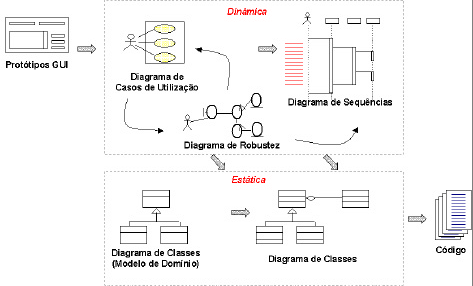
\includegraphics[scale=1.2]{./imagens/iconix1.png}}
%   \caption[Visão Geral do ICONIX]
%           {Visão Geral do ICONIX. \textbf{Fonte:} \cite{UML_Silva_Videira}}
% \label{fig:exemplo1}
% \end{figure}
% 
% \par A visão gerla do ICONIX pode ser exemplificada na figura 1, identificando a
% característica peculiar e a importância de utilizar o UML, levando em
% consideração que um sistema gera uma dependência de uma versão mais detalhada
% dos diagramas, isso porque é óbivio o uso destes diagramas para implementaçao do
% código.
% 
% \subsection{Análise de Requisitos}
% 
% \par Para realizar a análise de requisitos é necessário que seja realizado
% algumas atividades, as quais são descritas a seguir e inlustrado na figura 2.
% 
% \begin{figure}[h!]
%   \centerline{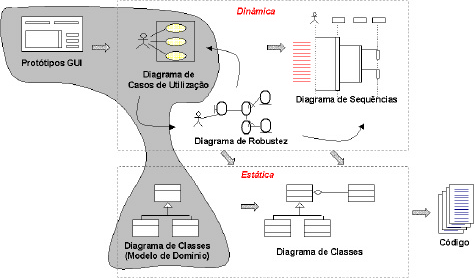
\includegraphics[scale=1.2]{./imagens/iconix2.png}}
%   \caption[Tarefa de análise de requisitos]
%           {Tarefa de análise de requisitos. \textbf{Fonte:}
%           \cite{UML_Silva_Videira}}
% \label{fig:exemplo1}
% \end{figure}
% 
% \begin{itemize}
%   \item Fazer com que seja identificados os objetos retirados da realidade,
%   assim como todo os atos de relatar compostos na generalização, associação e na
%   agregação. Utilizar também o digrama de modelo de domínio que coresponda ao
%   diagrama de classe em elevado escalão.
%   \item Ao notar orgaçamento suficiênte para desenvolvimento de protótipos que
%   utilizam uma interface gráfica ou GUI (\textit{Graphical User   Interface}), 
%   a utilização de digramas de navegação, facilitando o intendimento
%   do cliente e de seus usuários.
%   \item Fazer a identificação dos casos de utilização que estejam diretamente
%   ligados ao sistema. Elaborar o digrama de caso de utilização deixando em
%   evidência os atores e suas relações que estejam envolvidos.
%   \item Fazer um divisão organizada em conjuntos do casos de utilização,
%   separando estes conjuntos em digramas de pacotes (\textit{packages}).
%   \item Realizar a agremiação de requisitos funcionais com os casos de uso, e
%   criando vínculo com os objetos de domínio.
% \end{itemize}
% 
% \par No processo ICONIX, faz-se distinção clara de um requisito e um caso de
% utilização, de acordo com \citeonline[p.378]{UML_Silva_Videira} seguintes
% características peculiáres:
% 
% \begin{citacao}
%      \par Um caso de utilização descreve uma unidade de comportamento.
%   	 \par Um requisito descreve uma regra que governa o comportamento.
%   	 \par Um caso de utilização satisfaz um ou mais requisitos funcionais.
%   	 \par Um requisito funcional pode ser satisfeito por um ou mais casos de
% 			utilização.
% \end{citacao}
% 
% \par Assim o processo do ICONIX, tem relações de muitos para muitos no meio de
% casos de utilização e os requisitos.
% 
% \subsection{Análise e Desenho Preliminar}
% 
% \par Para realizar a análise e desenho preliminar é necessário que seja
% realizado algumas atividades, as quais são descritas a seguir e inlustrado na
% figura 3.
% 
% \begin{figure}[h!]
%   \centerline{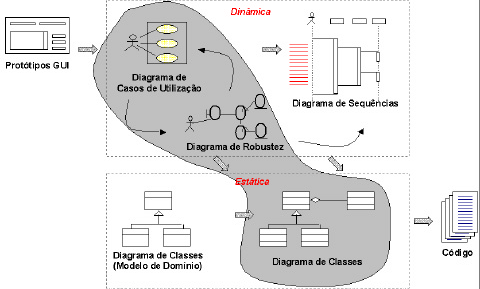
\includegraphics[scale=1.2]{./imagens/iconix3.png}}
%   \caption[Tarefa de análise e desenho preliminar]
%           {Tarefa de análise e desenho preliminar. \textbf{Fonte:}
%           \cite{UML_Silva_Videira}}
% \label{fig:exemplo1}
% \end{figure}
% 
% \begin{itemize}
%   			\item Descrever todos os casos de utilização que estivem ligados com os
%   			cenários alternativos, cenários de excepção e cenário principal.
%   			\item Elabora diagramas de análise de robustez. A cada diagrama de caso de
%   			utlização é necessário um diagrama de Robutez 
%   			
%   			\begin{itemize}
%   				\item Fazer a identificação primeiramente do conjunto de objetos,
%   				fazendo uso de estereótipos definidos pela UML(), que são as entidades
%   				(\textit{entity}), interface/fronteira (\textit{boundary}) e a de controle
%   				(\textit{control}), que são espeficados no ``processo de desenvolviemto de
%   				software``.
%   				\item Fazer a atualização relacionadas ao diagrama de domínio,
%   				introduzindo os novos objetos e atributos que foram gerados pelo processo
%   				de descoberta.			
% 			\end{itemize}
% 
%   			\item Fazer as atualizações no diagrama de classe de modo que repercuta
%   			seus resultados na finalização da fase de análise.
% \end{itemize}
% 
% \subsection{Desenho}
% 
% \par Para realizar o desenho é necessário que seja
% realizado algumas atividades, as quais são descritas a seguir e inlustrado na
% figura 4.
% 
% \begin{figure}[h!]
%   \centerline{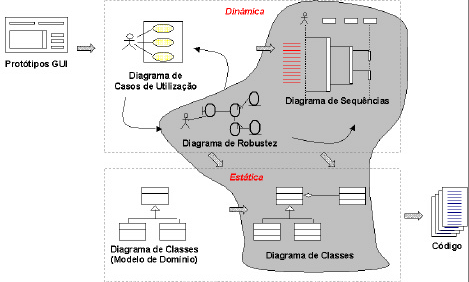
\includegraphics[scale=1.2]{./imagens/iconix4.png}}
%   \caption[Tarefa de Desenho]
%           {Tarefa de Desenho. \textbf{Fonte:}
%           \cite{UML_Silva_Videira}}
% \label{fig:exemplo1}
% \end{figure}
% 
% \begin{itemize}
%   \item Cada Caso de tiliação é necessário a a específicação do comportamento.
%  	
%  	\begin{itemize}
%  	  \item  Fazer identificação das mensagens que são enviadas e recebidas entre
%  	  métodos e objetos parceiro e que foram invocados, de modo a identificar os
%  	  objetos. O diagrama de sequência deve conter ao seu lado direio as
%  	  informações textuais do desenho e ao lado esquerdo as informações textuais
%  	  do caso de utilização. Continuar a atualização relacionadas ao diagrama de domínio,
%   	  introduzindo os novos objetos e atributos que foram gerados pelo processo
%   	  de descoberta.
%  	  \item Se for necessário pode-se usar digramas de colaboração como forma de
%  	  ilustrar as principais transações dos objetos.
%  	\end{itemize}
%  	
%  	\item Finalizar os diagramas que são do modelo estático, e incluir informações
%  	detalhadas sobre o diagrama, dentro da visibilidade e dos padrões do desenho.
%  	
% \end{itemize} 
% 
% 
% \subsection{Implementação}
% 
% \par Para realizar a implementação é necessário que seja
% realizado algumas atividades, as quais são descritas a seguir e inlustrado na
% figura 5.
% 
% \begin{figure}[h!]
%   \centerline{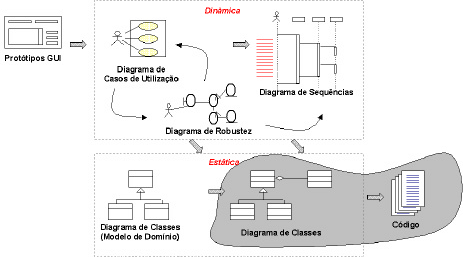
\includegraphics[scale=1.2]{./imagens/iconix5.png}}
%   \caption[Tarefa de Implementação]
%           {Tarefa de Implementação. \textbf{Fonte:}
%           \cite{UML_Silva_Videira}}
% \label{fig:exemplo1}
% \end{figure}
% 
% 
% \begin{itemize}
%   \item De acordo com as necessidade do projeto, deve-se elaborar diagramas de
%   arquitetura, como por exemplo diagramas de instalação e de componentes, que
%   ampare os estágios de implatanção.
%   \item Compor códificação e anotações.
%   \item Elaborar rotinas de testes, como o cárter unitário e de intergração.
%   \item Elaborar rotinas de testes, no sistema como um todo e com foco no
%   usuário, visando sua aceitação.
% \end{itemize} 




\chapter{QUADRO METODOLÓGICO}


\par Abordamos neste capítulo o método de pesquisa que foi utilizado para a
implementação deste projeto de pesquisa possibilitando sua conclusão.

\par Para \citeonline{Pesquisa_Santos_Candeloro},

\begin{citacao}
	A Expressão “método” remonta à Grécia antiga; methodos (methà + odon),
	siginifica “o caminho para se chegar a um fim”, legando-nos o emprego que
	hoje fazemos, o sentido de eleger um caminho a ser percorrido para se atingir
	um fim. Em se tratando de pesquisa cientifíca, são várias as possibilidades
	para executar uma invetigação e o fim almejado é o da comprovação ou refutação
	das hipóteses levantadas. Em primeiro lugar, deve-se considerar a área na qual
	o acadêmico está inserido e o tema com o qual pretende trabalhar. Após, devese
	construir um Referencial Teórico suficiente que permita o enuciado de um
	problema de pesquisa e suas respectivas variáveis.(p.69). 
\end{citacao}

\par Acompanhando o autor citado anteriormente, podemos concluir que a metodologia de
pesquisa bibliografica fornecera base para o desenvolvimento do projeto, apoiado no problema
de pesquisa e na resolução dos mesmos.

\section{Tipo de Pesquisa}

\par Na implementação do projeto, faz-se necessário a pesquisa que é o meio de 
gerar inovação e conhecimento, e através dela buscar respostas, para 
\citeonline{Pesquisa_Ciribelli}, A pesquisa torna-se fator chave, para a
veracidade e qualidade de um trabalho. Tornando-se assim essencial para o ganho
de conhecimento, bem como é de suma importância na instituição educacional.
  
\par Segundo \citeonline{Pesquisa_Padua}, a pesquisa pode ser definida como, a
meneira vastosa, como um meio de resolver questões não solvidas, exercendo averiguações e questionamentos através
destes meios, podemos assim formar o conhecimento, tornando assim possível o entendimento
da existência que é utilizada com base para ação.

\par Com base neste conceito, anteriormente citados, entende-se que a pesquisa é uma forma
de resolver problemas de pesquisa e gerar conhecimento, embasado neste princípio, a metodologia
aborda, tem como finalidade, apoiar meios de aperfeiçomanentos
do processo de elaboração do projeto .
%
%	*  Tipos de Pesquisa: ( Pesquisa Aplicada / Pesquisa de intervenção )
%	* 
%		* Definir a pesquisa
%		* O porquê da pesquisa
%		* de 3 a 4 paragráfos


\par A metodologia de pesquisa utilizada neste trabalho foi aplicada, onde o
principal foco deste tipo de pesquisa é a geração de conhecimento, dentro de um
espaço curto de tempo, propondo a aplicação prática da metodologia, tendo como
foco um meio de resolver um problema ou uma necessidade de maneira única, cujo o
problema tenha realação e participação com os ambientes locais e regionais.

%falta o tipo de pesquisa -ok 
\par Esta pesquisa utiliza como foco de pesquisa a pesquisa qualitativa, que
segundo \citeonline{Pesquisa_Demo} `` A pesquisa qualitativa busca apenas
realçar partes formalizando com jeito.''




% Contexto da pesquisa

\section{Contexto}

\par Para auxiliar à pesquisa forão utilizados livros, manuais, tutoriais,
trabalhos e artigos acadêmicos e páginas da internet. Utilizando tanto quanto 
para o embasamento teórico tanto quanto para o prático.

\par Com base nas pesquisas elaboradas, foi possível identificar que devido ao
grande volume de dados trafegados na rede, podemos assim complementa que se faz necessário gerir a rede.

\par Segundo \citeonline{Java_Costa_Avancado}, atualmente identificamos o crescimento das redes, bem como
suas estruturas que possui infraestrura complexa. O aumento consideravél de acessos a rede
mundial de computadores á um incitamento impulsionando a criação de novos meios de manter
operantes as rede dentro das condições esperadas.

\par Para \citeonline{Redes_Mosharraf_Forouza},

\begin{citacao}
	Podemos definir o gerenciamento de redes como a tarefa de testar, monitorar,
	configurar e resolver problemas dos componentes de rede com o obejtivo
	de atender um conjunto de requisitos definidos por uma organização. Esses
	requisitos incluem a operação regular e eficiente de rede, proporcionando a
	qualidade de serviços predefinida para os usuários. Para realizar essa tarefa,
	um sistema de gerenciamento de rede usa hardware, software e seres
	humanos.(p.693).
\end{citacao}

\par Conforme \citeonline{Java_Costa_Avancado}, A adminstração de rede é fundamentada na coleta direta de
informação, que constitui toda a estrutura. Com base nesta informações podemos análisar uma
ou mais rede de forma dinâmica, fazendo-se compreender através de seu estado atual.

% detalhes do local de desenvolvimento e de possível aplicação

\par O desenvolvimento da aplicação foi utilizado o eclipse na versão 4.4,
disponível para download no site www.eclipse.org, que é uma ferramenta de
desenvolvimento considerado com IDE (\textit{Integrated Development
Environment}).

%  Participantes : ( Lugar, o que faz, como vai ajudar, pra que serve )
\section{Participantes}

\par Este projeto é escrito por:
\par Israel José da Cunha
\par Graduando em Sistemas de Informação na UNIVAS - Universidade do Vale do
Sapucaí 
\par Professor de informática básica, Intermediária, avançada e aplicada na
Tecnologia.com - Escola Profissionalizante
\par Professor de Tecnologia da Informação no Estado de Minas Gerais - Escola
Estadual Professora Maria Vitorino de Souza.


\par Sob a arientação de:
\par Márcio Emílio Cruz Vono de Azevedo
\par Graduação em Engenharia Elétrica, modalidade Eletrônica pelo Inatel -
Instituto Nacional de Telecomunicações
\par Mestrado em Ciência e Tecnologia da Computação pela UNIFEI - Universidade
Federal de Itajubá
\par Professor no curso de Sistemas de Informação da UNIVÁS - Universidade do
Vale do Sapucaí
\par Professor no curso de Engenharia da Computação do Inatel - Instituto
Nacional de Telecomunicações
\par Especialista em Sistemas no Inatel - Instituto Nacional de Telecomunicações


\section{Instrumentos}

%	*  Instrumentos
%		* Reuniões
%			* Temática - Discussão do tema - Mais aberto permitindo o posicionamento das
%			% integrante * Entrevistas
%			* Estruturadas - Faz a pergunta ela dá a resposta e não mudança de assunto
%			% forçando isso.
%			* Semi Estruturadas -  Entre a estruturada e a aberta o meio termo
%			* Abertas - Totalmente Aberta

%		* Questionários 
%			* Fechados - Respostas em "x" 
%			* Abertos 
%			* Mistos

%Normalmente aplica-se o questionário depois as entrevistas e finalizando com a
% reunião para fechar as opiniões.

%Precisa aparecer no projeto:

%	* Qual o instrumento ?
%	* Qual a definição deste instrumento ? Ex: segundo lakato entrevista é ...
%	* Qual o objetivo do instrumento ? (O porquê do instrumento ?)
%	* Qual a periodicidade ?

\par A pesquisa é um meio de fomentar a coleta dedas, de acordo com
\citeonline{Pesquisa_Lakatos}, os instrumentos de pesquisa contém “desde os
tópicos da entrevista, passando pelo questionário e formulário, 
até os teste ou escala de medidas de opiniões e atitudes”.

% falta
% Instrumentos  -> O que foi usado para obter informações para o desenvolvimento ( Reuniões, entrevistas, questionários, editais, Etc. )
%	1. Definir o instrumento 
%	2. qual o objetivo deste instrumento
%	3. quantos
%	4. Cotucos no trabalho
%		1. Anexos ( Pego e Não modifico ) 
%		2. Apêndice ( Crio ou pego algo e modifico )

\par 


\subsection{Reunião}

\par Serão realizadas reuniões presenciais e virtuais com o professor
orientador, para a discussão dos requisitos, da usabilidade, 
dos processos de engenharia de software e desenvolvimento, questões 
teóricas sobre a aplicabilidade e a orientação para o desenvolvimento do
projeto, será também feito reunião com pessoas que atuam na área para coletar
experiência de campo.

\par Todas as reuniões terão cárter aberto, para livre habitrio dos
participantes.


\par Toda á pesquisa do projeto serão fundamentados em livros, artigos
científicos e acervos digitais.

\par Para \citeonline{Projetos_Cabanis-brewin},
\begin{citacao}
	Documentos incluem planos, registros administrativos, dados técnicos, documentos
	de engenharia e construção, procedimentos, documentos sobre o sistema,
	relatórios e correspondências. Esta seção do plano de gerenciamento do
	projeto identifica os documentos que serão preparados no projeto e estabelece
	a abordagem administrativa, sistemas e procedimentos a serem utilizados para
	gerenciar essa documentação.(p.62)
\end{citacao}

\par A documentação é parte do trabalho, que formula os meios usados no decorrer do projeto,
facilitando a geração de relatórios e emplementação dos requisitos.


\subsection{Metodologia de Desenvolvimento}

\par Será utilizado o modelo de processo chamado ICONIX, por ser um modelo de desnvolvimento
de software iterativo e incremental.

\par De acordo com \citeonline{UML_Silva_Videira}, O ICONIX trata-se de um método de desenvolvimento
de Software, que é divido em quatro pequenos grupo de trabalho, que possuem tempo
de execução. As divisões são: Análise de requisitos, análise e desenho preliminar, desenpenho
e implementação.

\par Ainda segundo \citeonline{UML_Silva_Videira}, Esta metodologia compoem-se em
produzir uma gama de produtos, que descreve com exatidão na perspectiva do sistema, utilizado de meios
incrementais e paralelos, apresentando o ponto de vista Dinâmico e Estático.


\section{Procedimentos}
%   Procedimentos 
%	* Passo-a-passo para o desenvolvimento do software.
%		* Imaginar tudo que vai ter que fazer para fazer o sistema
%			* Todas as ações que poderão ser desenvolvidas
%			* Em tópicos
%			* Em ordem cronológica

% 			FALTA
%Procedimento
%	1. Descrever as ações realizadas para o desenvolvimento
%	2. Descritivo e Detalhado 
%	3. Passo a passo o que foi feito

\begin{itemize}
  \item Análise de Requisitos - Elaboração do plano de execução do projeto de
  desenvolvimento de software.
  \item Implementação do ICONIX - Elaboração dos Digramas de Sistema
  	
  	\begin{itemize}
 	 	\item Análise de requisitos
  		\item Análise e desempenho preliminar
  		\item Desenhos
  		\item Implementação
	\end{itemize}
  	
  \item Revisão do ICONIX
  \item Codificação do projeto 
  \item Teste de codficação 
\end{itemize}

\par O desenvolvimento do aplicativo foi baseado na tecnologia JAVA, através da
IDE Eclipse, o aplicativo tem como finalidade o gerenciamento de dados na rede
de computadores, este tem usabilidade de apresentar graficos e meios de
verificar os resultados de transferências de dados e aplicações que estejam em
execução no instante de seu respectivo uso.

\par Foi elaborado as fases do ICONIX, que são as seguintes, Análise de
requisitos, Análise e desempenho preliminar e os diagramas.

\par Após a criação dos digramas deu-se início ao desenvolvimento da aplicação,
através da Linguagem de programação JAVA.


%\section{Resultados}

%Resultados
%	1. O que foi obtido a partir das ações ( Descritivo e detalhado )

%Poder fazer isso -> Procedimentos e Resultado
%	1. Exceto tipo de pesquisa as outras seções deverão estar no tempo verbal
	% "PASSADO" 2. Texto Técnico porém científico
% Pode usar em formato de tabela.

%\par Os resoltados demonstram que para cada ação feita existe um resultado
%equivalente. Na tabela á seguir estão exemplificados todas as ações feitas.

%\begin{small}
%\begin{tabular}{clr}
%\hline
% Procedimento & Resultados  \\
%\hline
% 	1-  & 1-  \\
% 	2- & 2-  \\
% 	3-  & 3-   \\
% 	4-   & 4-  \\ 
% 	5-  & 5-  \\ 
%\hline
%\end{tabular}


%\end{small}





% Cronograma

\section{Cronograma}

\begin{table}[!htpb]
\centering

% definindo o tamanho da fonte para small
% outros possíveis tamanhos: footnotesize, scriptsize
\begin{small} 
  
% redefinindo o espaçamento das colunas
\setlength{\tabcolsep}{8pt} 

% \cline é semelhante ao \hline, porém é possível indicar as colunas que terão essa a linha horizontal
% \multicolumn{10}{c|}{Meses} indica que dez colunas serão mescladas e a palavra Meses estará centralizada dentro delas.

\begin{tabular}{|l|c|c|c|c|c|c|c|c|c|}\hline

\textbf{Ações / Meses} & Jun & Jul & Ago & Set & Out & Nov & Dez
\\
\hline

Qualificação & X &  &  &  &  &  &  \\ \hline

Redação do quadro teórico & X & X &  &  &  &  &  \\ \hline

Redação do quadro metodológico & X & X & X &  &  &  &  \\ \hline

Desenvolvimento do sistema & X & X & X & X & X & X & X \\ \hline

Redação da discussão dos resultados & X & X & X & X & X & X & X \\ \hline

Pré-banca &  &  &  &  &  & X &  \\ \hline

Redação da introdução e considerações finais &  &  & X & X &  &  & \\\hline

Formatação final &  &  &  &  &  & X & X \\ \hline

Banca de defesa &  &  &  &  &  &  & X \\ \hline

Correções finais &  &  &  &  &  &  & X \\ \hline

Entrega de Capa Dura &  &  &  &  &  &  & X \\ \hline

Reuniões & X & X & X & X & X & X & X \\ \hline

Revisões Bibliograficas & X & X & X & X & X & X & X \\ \hline

Revisão Textual & X & X & X & X & X & X & X \\ \hline


\end{tabular} 
\end{small}
\caption{Cronograma das atividades previstas}
\label{t_cronograma}
\end{table} 


\section{Orçamento}

% Orçamento
%	* Listar todas as despesas com o TCC
%		* Folhas 
%		* Tintas
%		* Encadernação
%		* Internet
%		* Transporte
%		* Capa Dura
%		* Estipular um valor médio ( não ficar muito baixo e nem muito auto )



\begin{small}
\begin{tabular}{clr}
\hline
 Despesas & Valor Previsto (R\$)   \\
\hline
 	Impressão & R\$ 150,00  \\
 	Encadernação & R\$ 70,00  \\
 	Impressão Capa Dura  & R\$ 200,00  \\
 	Livros  & R\$ 475,00  \\ 
 	Ebook  & R\$ 254,00  \\ \hline
 	\textbf{Total} & \textbf{R\$ 1.149,00} \\
\hline
\end{tabular}


\end{small}


% Descritivo detalhado

%\par

















%\chapter{CRONOGRAMA}

\par Fazer o cronograma do projeto
%\chapter{ORÇAMENTO}

\par fazer Orçamento do projeto
%
\chapter{DISCUSÃO RESULTADOS} 

\par Este capítulo tem por finalidade representar e na integra o que foi
observado durante o desenvolvimento do trabalho e as dificuldades de pesquisa,
de desenvolvimento e diagramação.

\par Será inseridos também os dasafios que foram enfrentados para realização do
projeto.


\par De acordo com a pesquisa realizada o SNMP é essencial para o gerenciamento
de de redes, com foco no dispositivos que estejam conectados.

Segundo \citeonline{SNMP_Schmidt_Mauro}

\begin{citacao}
	O núcleo do SNMP é um conjunto simples de operaçãoes(e das informações obtidas
	por essas operações) que permitem ao administrador modificar o estado de alguns
	dispositivos baseados em SNMP. Por exemplo, é possível utilizar o SNMP para
	encerrar uma interfaceem roteador ou verificar a velocidade operacional de uma
	interface de Ethernet.
\end{citacao}


\par Devido ao grande volume de dados trafegados na rede, podemos assim complementa
que se faz necessário gerir a rede.

\par Segundo \citeonline{Java_Costa_Avancado}, atualmente identificamos o crescimento das redes, bem como
suas estruturas que possui infraestrura complexa. O aumento consideravél de acessos a rede
mundial de computadores á um incitamento impulsionando a criação de novos meios de manter
operantes as rede dentro das condições esperadas.

\par Para \citeonline{Redes_Mosharraf_Forouza},

\begin{citacao}
	Podemos definir o gerenciamento de redes como a tarefa de testar, monitorar,
	configurar e resolver problemas dos componentes de rede com o obejtivo
	de atender um conjunto de requisitos definidos por uma organização. Esses
	requisitos incluem a operação regular e eficiente de rede, proporcionando a
	qualidade de serviços predefinida para os usuários. Para realizar essa tarefa,
	um sistema de gerenciamento de rede usa hardware,software e seres humanos.(p.693).
\end{citacao}

\par Conforme \citeonline{Java_Costa_Avancado}, A adminstração de rede é fundamentada na coleta direta de
informação, que constitui toda a estrutura. Com base nesta informações podemos análisar uma
ou mais rede de forma dinâmica, fazendo-se compreender através de seu estado atual.

\par Para \citeonline{Projetos_Cabanis-brewin},
\begin{citacao}
	Documentos incluem planos, registros administrativos, dados técnicos, documentos
	de engenharia e construção, procedimentos, documentos sobre o sistema,
	relatórios e correspondências. Esta seção do plano de gerenciamento do
	projeto identifica os documentos que serão preparados no projeto e estabelece
	a abordagem administrativa, sistemas e procedimentos a serem utilizados para
	gerenciar essa documentação.(p.62)
\end{citacao}

\par A documentação é parte do trabalho, que formula os meios usados no decorrer do projeto,
facilitando a geração de relatórios e emplementação dos requisitos.

\par As imagens abaixo mostram como é a arquitetura utilizada na biblioteca
utilizada no java cujo é nomeada de snmpv4.



\begin{figure}[h!]
  \centerline{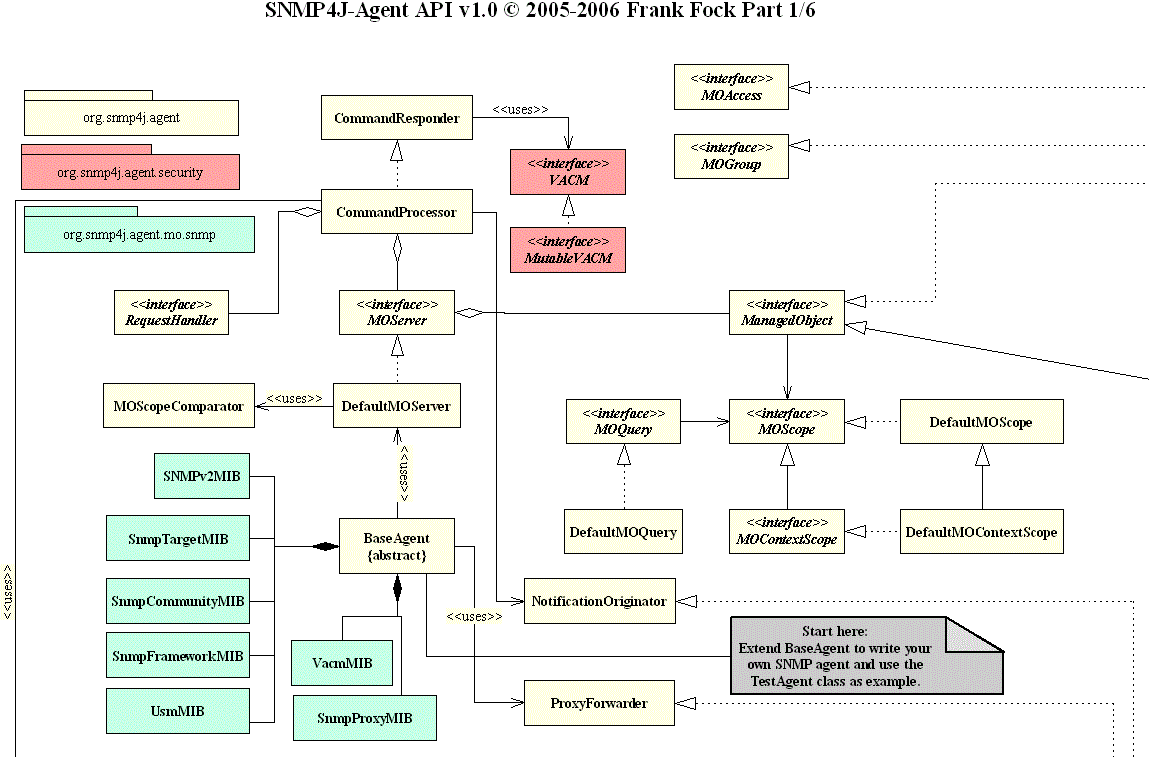
\includegraphics[scale=0.55]{./imagens/one.png}}
  \caption[Exemplo de criação de um projeto Web no Eclipse]
          {SNMP4J Client. \textbf{Fonte: snmp4j}
          \cite{Diagrama_do_SMNP4J}}
\label{fig:exemplo1}
\end{figure}





\begin{figure}[h!]
  \centerline{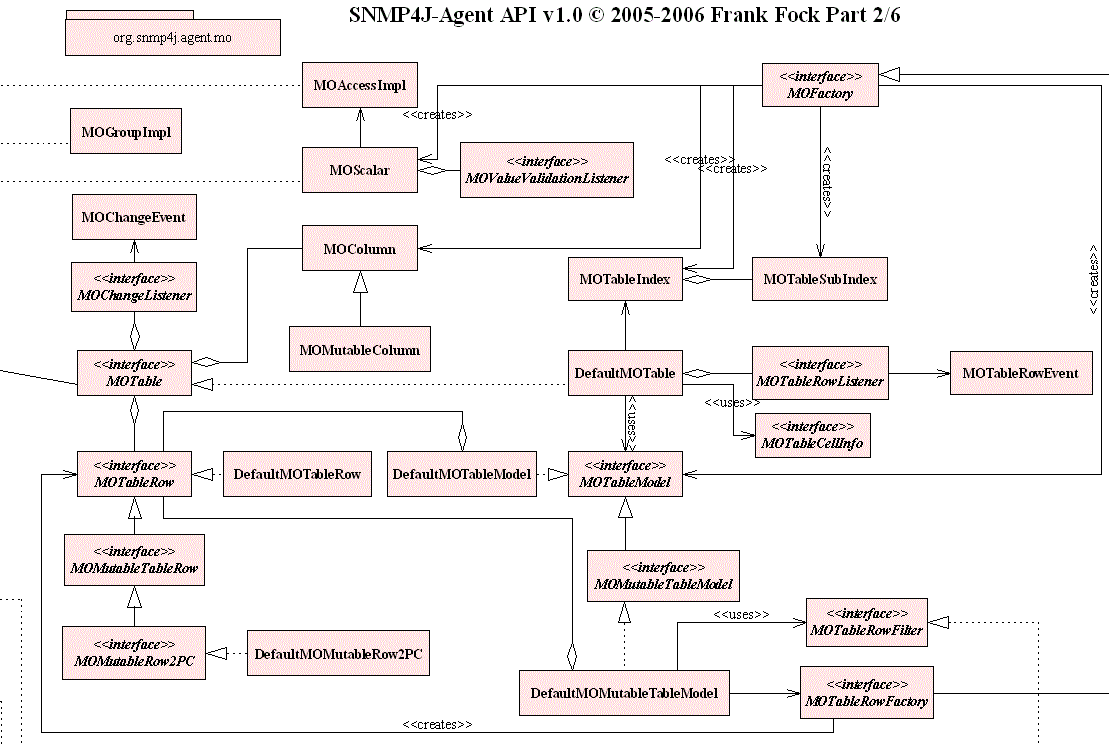
\includegraphics[scale=0.55]{./imagens/two.png}}
  \caption[Exemplo de criação de um projeto Web no Eclipse]
          {SNMP4J Client. \textbf{Fonte: snmp4j}
          \cite{Diagrama_do_SMNP4J}}
\label{fig:exemplo1}
\end{figure}




\begin{figure}[h!]
  \centerline{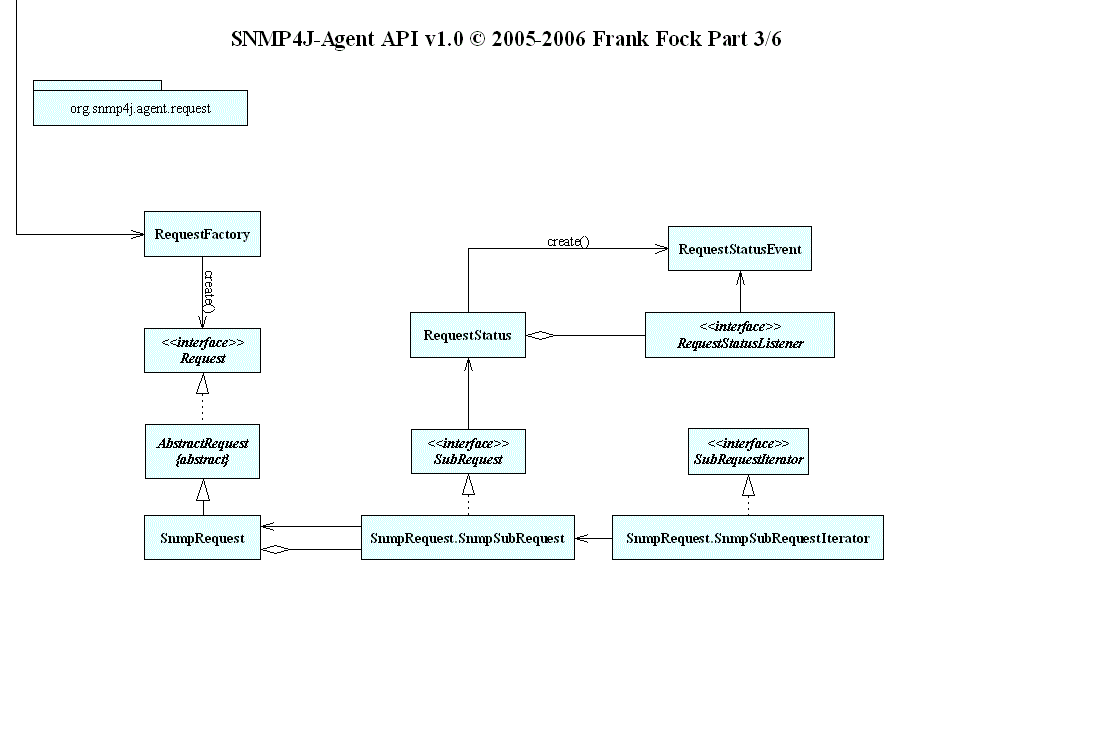
\includegraphics[scale=0.55]{./imagens/tres.png}}
  \caption[Exemplo de criação de um projeto Web no Eclipse]
          {SNMP4J Client. \textbf{Fonte: snmp4j}
          \cite{Diagrama_do_SMNP4J}}
\label{fig:exemplo1}
\end{figure}





\begin{figure}[h!]
  \centerline{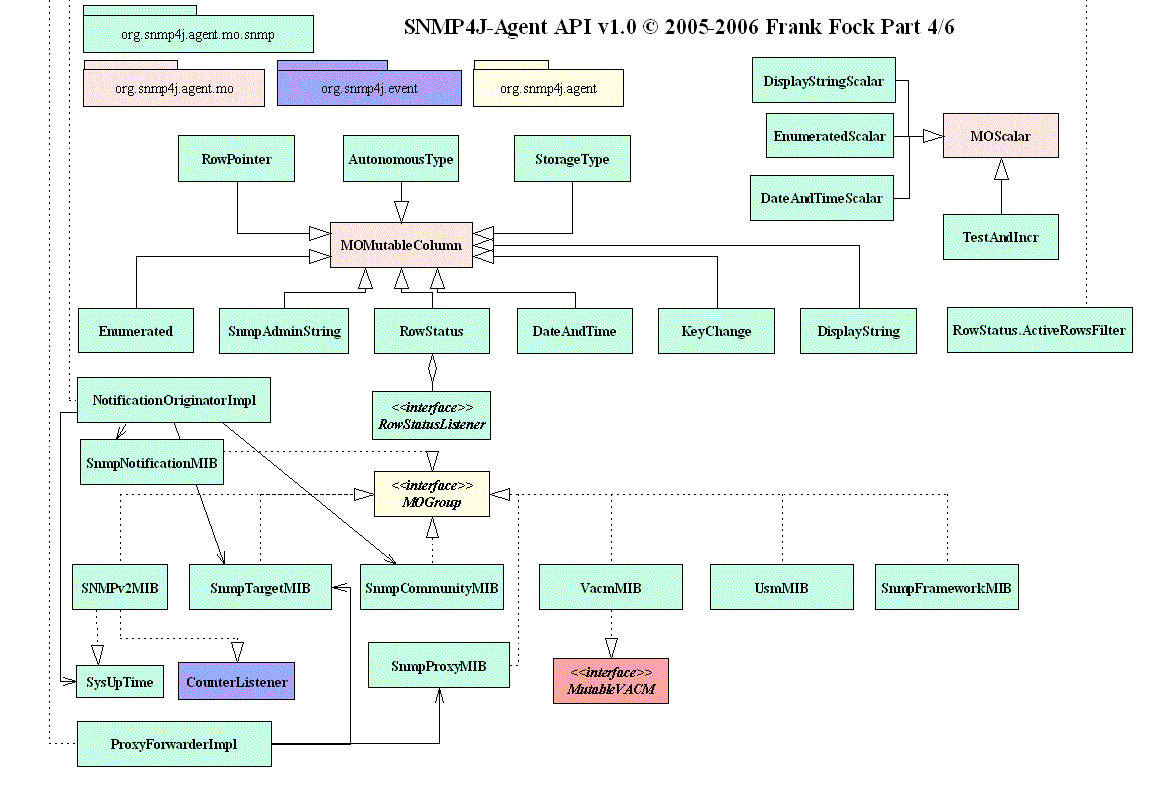
\includegraphics[scale=0.55]{./imagens/four.png}}
  \caption[Exemplo de criação de um projeto Web no Eclipse]
          {SNMP4J Client. \textbf{Fonte: snmp4j}
          \cite{Diagrama_do_SMNP4J}}
\label{fig:exemplo1}
\end{figure}




\begin{figure}[h!]
  \centerline{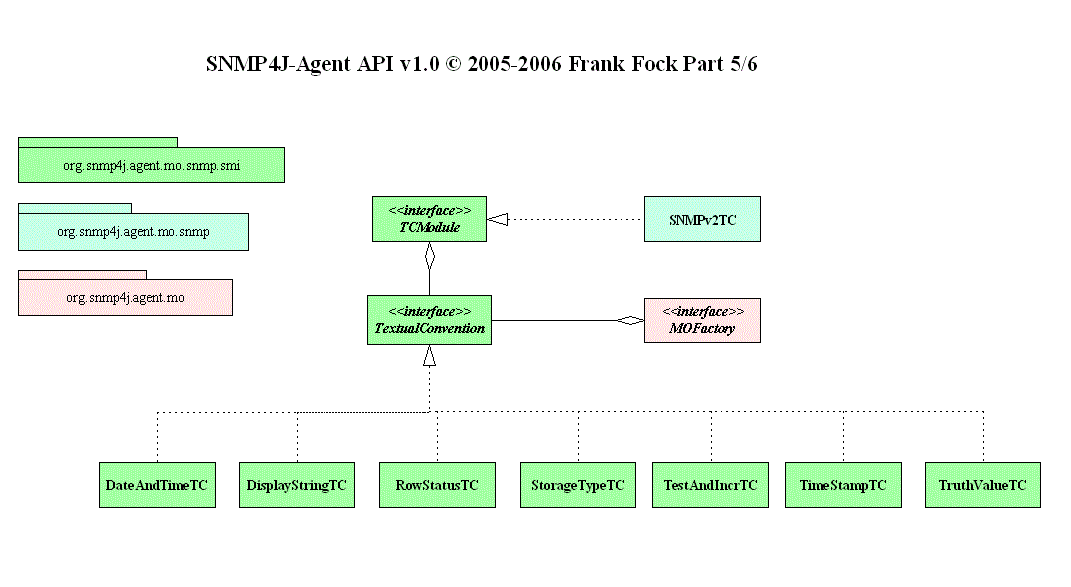
\includegraphics[scale=0.55]{./imagens/five.png}}
  \caption[Exemplo de criação de um projeto Web no Eclipse]
          {SNMP4J Client. \textbf{Fonte: snmp4j}
          \cite{Diagrama_do_SMNP4J}}
\label{fig:exemplo1}
\end{figure}



\begin{figure}[h!]
  \centerline{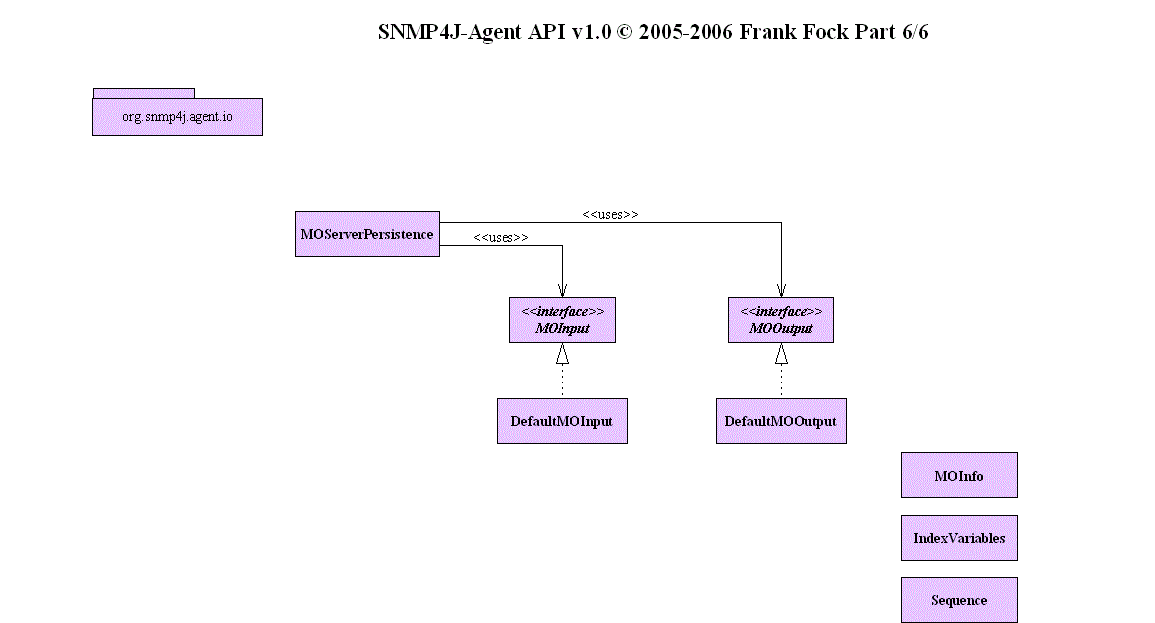
\includegraphics[scale=0.55]{./imagens/six.png}}
  \caption[Exemplo de criação de um projeto Web no Eclipse]
          {SNMP4J Client. \textbf{Fonte: snmp4j}
          \cite{Diagrama_do_SMNP4J}}
\label{fig:exemplo1}
\end{figure}



%
\chapter{CONCLUSÃO} 

\par A conclusão deste trabalho é \ldots

\par Assim conclui-se que \ldots





\postextual %Início dos Elementos Pós-Textuais

\bibliography{biblio}			            % insere as REFERENCIAS (arquivo biblio.bib)
\addcontentsline{toc}{chapter}{REFERÊNCIAS} % adiciona o título no sumário

%\begin{apendicesenv}

%\apendicesname{APÊNDICES}
% Imprime uma página indicando o início dos apêndices
\partapendices*

\addcontentsline{toc}{chapter}{APÊNDICES}

\chapter*{Título do Apêndice I}
\label{apendice:1}

\par Aqui deve conter o texto do Apêndice~\ref{apendice:1}. Na Figura~\ref{fig:ap1:identificador} é ilustrada a primeira tela deste processo.
\captionsetup[figure]{list=no}
\begin{figure}[h!]
 \centerline{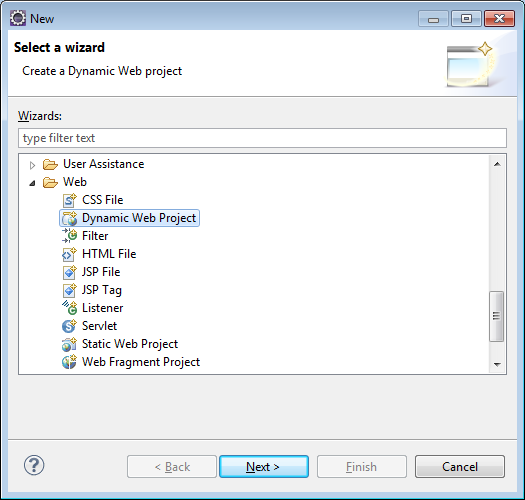
\includegraphics[scale=0.5]{./imagens/apendice_img1.png}}
 \caption[Outra imagem.]
           {Outra imagem. \textbf{Fonte:} Elaborado pelos autores}
  \label{fig:ap1:identificador}
\end{figure}

\par Após a seleção do tipo de projeto \ldots
\chapter*{Título do Apêndice 2}

\section*{Primeira seção do apêndice 2}

\par Neste apêndice é mostrado \ldots de acordo com a Figura~\ref{fig:ap2:identificador} é ilustrada a primeira tela deste processo.
\captionsetup[figure]{list=no}
\begin{figure}[h!]
 \centerline{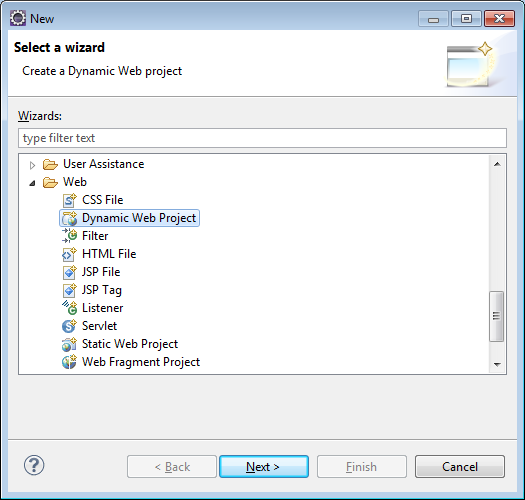
\includegraphics[scale=0.3]{./imagens/apendice_img1.png}}
 \caption[Outra imagem ainda.]
           {Outra imagem ainda. \textbf{Fonte:} Elaborado pelos autores}
  \label{fig:ap2:identificador}
\end{figure}

\section*{Segunda seção do apêndice 2}


\par Continuando \ldots na figura Figura~\ref{fig:xml_exemplo} é mostrado um exemplo de XML.

\begin{figure}[h!]
\begin{lstlisting}[style=custom_XML]
<project>
...
 <dependencies>
  ...
  <dependency>
   <groupId>org.neo4j</groupId>
   <artifactId>neo4j</artifactId>
   <version>1.9.4</version>
  </dependency>
  ...
 </dependencies>
 ...
</project>
\end{lstlisting}  
 \caption[Exemplo de código XML.]
           {Exemplo de código XML. \textbf{Fonte:} Elaborado pelos autores}
  \label{fig:xml_exemplo}
\end{figure}



\end{apendicesenv}
%%\anexoname{ANEXOS}
%\begin{anexosenv}
%\partanexos
%\chapter*{ANEXO I}

%\end{anexosenv}

\addcontentsline{toc}{chapter}{ANEXOS}

\chapter*{ANEXO I}



\printindex

\end{document}